%import template

\documentclass[a4paper, landscape , 8pt]{scrartcl}

% use language german
\usepackage[T1]{fontenc}
\usepackage[utf8]{inputenc}
\usepackage[english, ngerman]{babel} % \selectlanguage{english} if  needed
\usepackage{lmodern} % use modern latin fonts

% format
\usepackage{geometry}
\geometry{top=1.2cm,left=0.4cm,right=0.4cm}

%autor
\usepackage{authblk}

% math
\usepackage{amsmath}
\usepackage{amssymb}
\usepackage{amsfonts}
\usepackage{enumitem}

% graphic
\usepackage{graphicx}
\graphicspath{{graphic/}} 

%colors
\usepackage{xcolor}

% Multi Columns
\usepackage{multicol}

%compact items
\usepackage{paralist}

%define header and footer
\usepackage{fancyhdr}
\pagestyle{fancy}

\fancyhead[RO]{Zindel Marius}
\fancyhead[LO]{\TITLE}
\fancyfoot[RO]{29.08.2020}
\fancyfoot[LO]{Created with \LaTeX}
\renewcommand\headrulewidth{0pt}
\renewcommand\footrulewidth{0pt}
\headsep = -9pt
\footskip = 0pt
\textheight = 563pt

%define section color and size
\addtokomafont{section}{\color{sectioncolor}\small\rule{\linewidth}{.5pt}\vspace{-2pt}\\}
\addtokomafont{subsection}{\color{subsectioncolor}\small}
\addtokomafont{subsubsection}{\color{subsubsectioncolor}\small}

%no section numbers
\setcounter{secnumdepth}{0}

%define section spacing
\RedeclareSectionCommands[ 
	afterindent = false, 
	beforeskip = 0pt, 
	afterskip = .1pt 
	]{section,subsection,subsubsection}

%define color
\definecolor{sectioncolor}{RGB}{1, 101, 163}
\definecolor{subsectioncolor}{RGB}{1, 101, 163}
\definecolor{subsubsectioncolor}{RGB}{0, 0, 0}
\definecolor{b}{RGB}{0, 120, 255} %Default highlite color
\definecolor{p}{RGB}{0, 43, 54} %Dark page color
\definecolor{t}{RGB}{131, 148, 150} %Dark text color
\definecolor{darkgreen}{RGB}{0,150,0}
\definecolor{dkgreen}{rgb}{0,0.6,0}
\definecolor{gray}{rgb}{0.5,0.5,0.5}
\definecolor{mauve}{rgb}{0.58,0,0.82}
\definecolor{DarkPurple}{rgb}{0.4, 0.1, 0.4}
\definecolor{DarkCyan}{rgb}{0.0, 0.5, 0.4}
\definecolor{LightLime}{rgb}{0.3, 0.5, 0.4}
\definecolor{Blue}{rgb}{0.0, 0.0, 1.0}
\definecolor{h}{RGB}{1, 101, 163}

% Code Listings
\usepackage{listings}
\usepackage{color}
\usepackage{beramono}
\usepackage{hyperref}
\hypersetup{
    colorlinks,
    linkcolor={black},
    citecolor={blue!50!black},
    urlcolor={blue!80!black}
}

\definecolor{bluekeywords}{rgb}{0,0,1}
\definecolor{greencomments}{rgb}{0,0.5,0}
\definecolor{redstrings}{rgb}{0.64,0.08,0.08}
\definecolor{xmlcomments}{rgb}{0.5,0.5,0.5}
\definecolor{types}{rgb}{0.17,0.57,0.68}

\lstdefinestyle{visual-studio-style}{
	language=[Sharp]C,
	basicstyle=\ttfamily\scriptsize,
	columns=flexible,
	showstringspaces=false,
	basicstyle=\footnotesize\ttfamily, 
	commentstyle=\color{greencomments},
	morekeywords={partial, var, value, get, set},
	keywordstyle=\bfseries\color{bluekeywords},
	stringstyle=\color{redstrings},
	breaklines=true,
	breakatwhitespace=true,
	tabsize=4,
	numbers=none,
	numberstyle=\tiny\color{black},
	frame=none,
	showspaces=false,
	showtabs=false,
	escapeinside={£}{£},
}

\lstdefinestyle{cevelop-style}{
	language=C++,
	basicstyle=\ttfamily\scriptsize,
	columns=flexible,
	showstringspaces=false,     
	basicstyle=\footnotesize\ttfamily, 
	keywordstyle=\bfseries\color{DarkPurple},
	commentstyle=\color{LightLime},
	stringstyle=\color{Blue}, 
	escapeinside={£}{£}, % latex scope within code      
	breaklines=true,
	breakatwhitespace=true,
	showspaces=false,
	showtabs=false,
	tabsize=4,
	morekeywords={include,ifndef,define},
	numbers=none,
	numberstyle=\tiny\color{black},
	frame=none,
}

\lstdefinestyle{eclipse-style}{
	language=C,
	showstringspaces=false,     
	basicstyle=\ttfamily\scriptsize,
	keywordstyle=\color{blue}\ttfamily,
    stringstyle=\color{red}\ttfamily,
	commentstyle=\color{darkgreen}\ttfamily,
	escapeinside={£}{£}, % latex scope within code      
	breaklines=true,
	breakatwhitespace=true,
	showspaces=false,
	showtabs=false,
	tabsize=4,
	morekeywords={length},
	numbers=none,
	numberstyle=\tiny\color{black},
	frame=top,
}
\lstset{style=eclipse-style}

% Theorems \begin{mytheo}{title}{label}
\usepackage{tcolorbox}
\tcbuselibrary{theorems}
\newtcbtheorem[number within=section]{definiton}{Definition}%
{fonttitle=\bfseries}{def}
\newtcbtheorem[number within=section]{remember}{Merke}%
{fonttitle=\bfseries}{rem}
\newtcbtheorem[number within=section]{hint}{Hinweis}%
{fonttitle=\bfseries}{hnt}

% new section -> new page
% \let\stdsection\section
% \renewcommand\section{\clearpage\stdsection}

% Front page
\newcommand{\AUTHOR}{Marius Zindel}
\newcommand{\INSTITUTE}{Hochschule für Technik Rapperswil}

%dotted rule
\usepackage{dashrule}
\usepackage{tikz}
\usetikzlibrary{decorations.markings}
\newcommand{\drule}[3][0]{
	\tikz[baseline]{\path[decoration={markings,
	mark=between positions 0 and 1 step 2*#3
	with {\node[fill, circle, minimum width=#3, inner sep=0pt, anchor=south west] {};}},postaction={decorate}]  (0,#1) -- ++(#2,0);}}


%no indentation
\setlength{\parindent}{0cm}

% DocInfo
\newcommand{\SUBJECT}{}
\newcommand{\TITLE}{Cheat Sheet Bsys2}

\begin{document}

%import front page
%
\begin{titlepage}


\vspace*{\fill}

\newcommand{\HRule}{\color{sectioncolor}\rule{\linewidth}{0.5mm}} % Defines a new command for the horizontal lines, change thickness here

\center


\includegraphics[scale=.4,keepaspectratio]{Graphic/HSR_Logo_RGB_72}\\[1cm] 


\textsc{\huge \SUBJECT}\\[1cm]

{\HRule} \\[0.7cm]
{ \Huge \bfseries \textcolor{sectioncolor}{\TITLE}}\\[0.4cm]
{\HRule} \\[1.1cm]

\Large \AUTHOR

\Large 29.08.2020


\vfill % Fill the rest of the page with whitespace

\end{titlepage} 






\begin{multicols*}{5}
    \setlength{\columnseprule}{0.4pt}
        \footnotesize

% 
%Table of contents
\tableofcontents

% don't show \subsubsection in \tableofcontents
\setcounter{tocdepth}{2}

\section{Hex}
\begin{tabular}{r  r  r | r r}
		dec & hex& $2^x$& IT& $2^x$\\
		\hline
			32&20&$2^5$&K&$2^{10}$\\
			64&40&$2^6$&M&$2^{20}$\\
			128&80&$2^7$&G&$2^{30}$\\
			256&100&$2^8$&T&$2^{40}$\\
			512&200&$2^9$&P&$2^{50}$\\
			1024&400&$2^{10}$
		\end{tabular}
		
		\vspace{-1pt}
		
\section{Betriebsystem-API}

    \begin{compactitem}[$\bullet$]
        \item Abstraktion und damit Portabilität
        \begin{compactitem}
            \item von der Hardware, Protokollen, Software
        \end{compactitem}
        \item Ressourcenmanagement und Isolation der Anwendungen voneinander
        \begin{compactitem}
            \item Rechenzeit
            \item Hauptspeicherverwendung
            \item Sekundärer Speicher, Netzwerkbandbreite, etc.
        \end{compactitem}
        \item Benutzerverwaltung und Sicherheit
    \end{compactitem}


    \subsubsection{Kernel Mode}
    \begin{compactitem}[$\bullet$]
		\item OS: Prozessor mit mind. 2 Privilege Levels:
		\begin{compactitem}
			\item \textcolor{h}{Kernel-Mode:} Darf jede Instruktion
			\item \textcolor{h}{User-Mode:} Darf nur beschränkte Menge
		\end{compactitem}
		\item OS läuft im Kernel Mode und kann bestimmen, welche Software in welchem Modus läuft.
		\item Hardware-Mechanismus, um Applikationen voneinander zu isolieren
    \end{compactitem}
    
    \subsubsection{\texttt{syscall}}
    
    Mit \texttt{syscall}-Befehlt kann dem OS ein Kernelwechstel / Exit Code gesendet werden.
    Applikationen sollen nicht direkt Syscalls aufrufen, sondern C-Wrapper-Funktionen.
    
	\subsubsection{Programmargumente der Shell}
        \begin{compactitem}[$\bullet$]
            \item Shell teilt Programmargumente in Strings
            \item Leerzeichen als Trennung zwischen Argumenten
        \end{compactitem}
    
    
    \subsubsection{Calling Convention für Programmargumente}
		\begin{compactitem} [$\bullet$]
			\item Bei Start schreibt OS Argumente als null-terminierte Strings in Speicher
			\item \texttt{argv} $\rightarrow$ Array $\rightarrow$ 1. Zeichen Argumentes
			\item \texttt{argv[0]} ist der Programmname
        \end{compactitem}
    
        \subsubsection{Umgebungsvariablen}
            \begin{compactitem}[$\bullet$]
                \item Key - Value Paar mit =
                \item Key nur einmal vorkommen!
                \item Unter C zeigt die Variable \texttt{environ} auf Array
                \item \texttt{environ} nicht direkt verwendet, nur über: \texttt{getenv, putenv, setenv,} \texttt{unsetenv}
            \end{compactitem}        
			
			\vspace{-6pt}
            \begin{lstlisting}
//Abfragen einer Umgebungsvariable
char * getenv (const char * key);
//Setzen einer Umgebungsvariable                
int setenv(const char *key, const char *value, int overwrite);
//Entfernen einer Umgebungsvariable                
int unsetenv(const chat * key);
//Hinzufuegen einer Umgebungsvariable
int putenv(char * kvp);
			\end{lstlisting}
			\vspace{-6pt
			}
		Umgebungsvariablen werden dem Programm implizit bereitgestellt. Das ist nützlich, wenn Informationen normalerweise über alle Aufrufe gleich sind (z.B. Pfade).\\
	
		\vspace{-10pt}

\section{Dateisysteme}
	\textcolor{h}{Verzeichnis:} Datei mit Liste aller Dateien\\
    \textcolor{h}{Verzeichnishierarchie:} Baumstruktur aller Verzeichnisse im System\\
    \textcolor{h}{Wurzelverzeichnis:} root directory $\rightarrow$ /\\
    \textcolor{h}{Kanonische Pfade:} Ohne . und .. $\rightarrow$ realpath\\
    \textcolor{h}{Absolute Pfade:} beginnen bei / (Wurzelverz.)\\
    \textcolor{h}{Relative Pfade:} beginnen nicht bei / ! (beziehen sich auf Arbeitsverzeichnis)

    \subsubsection{Permission-Bits}
        0:none, 1:x , 2:w, 3:wx, 4:r, 5:rx, 6:rw, 7:rwx\\
		0740 oder rwxr - - - - - (9 Permission-Bits)








	\subsubsection{POSIX API}
	$\rightarrow$ für direkten Zugriff (Daten sind Binärdaten)
	
	\begin{compactitem}[$\bullet$]
		\item \textcolor{h}{errno} globale int Variable
		\item \textcolor{h}{strerror} gibt \textcolor{h}{Adresse} zurück auf String der Fehlercode beschreibt
		\item \textcolor{h}{perror} schreibt text + Ergebnis (von strerror(errno)) auf dem Error-stream
	\end{compactitem}
		
	\subsubsection{File-Descriptor}
		\begin{compactitem}[$\bullet$]
			\item \textcolor{h}{File-Descriptor} fd $\rightarrow$ Indize in eine globale Tabelle pro Prozess
			\item \textcolor{h}{File-Deskriptor-Tabelle} alle geöffneten Dateien vom Prozess, Index auf systemweite Tabelle, Zustandsbehaftet (read-offset)
			\item \textcolor{h}{Global-Descriptor-Table} enthält Daten um physische Datei zu identifizieren (Treiber, Datenträger, etc.)
		\end{compactitem}
		
		\vspace{-6pt}
		\begin{lstlisting}
int open (char *path, int flags, ...)
		\end{lstlisting}
		\vspace{-6pt}
		\begin{compactitem}[$\bullet$]
			\item Erzeugt einen File-Deskriptor auf die Datei, die an \texttt{path} liegt
			\item \texttt{flags} gibt an, wie die Datei geöffnet (rw)
		\end{compactitem}
		
		\vspace{-6pt}
		\begin{lstlisting}
int close (int fd);
		\end{lstlisting}
		\vspace{-6pt}
		\begin{compactitem}[$\bullet$]
			\item Dealloziert dem File-Deskriptor fd
		\end{compactitem}
			
		\vspace{-6pt}
		\begin{lstlisting}
ssize_t read(int fd, void * buffer, size_t n)
		\end{lstlisting}
		\vspace{-6pt}
		\begin{compactitem}[$\bullet$]
			\item Versucht die nächsten n Byte am aktuellen Offset von fd in den Buffer zu kopieren
			\item Gibt die Anzahl gelesener Bytes zurück	
			\item Erhöht Offset von fd um n
		\end{compactitem}

		\vspace{-6pt}
		\begin{lstlisting}
ssize_t write(int fd, void *buffer, size_t n)
		\end{lstlisting}
		\vspace{-6pt}
		\begin{compactitem}[$\bullet$]
			\item Versucht die nächsten n Byte vom buffer an den aktuellen Offset fd zu kopieren
			\item Gibt Anzahl geschriebener Bytes zurück
			\item Erhöht Offset fd um Anzahl geschrieben Bytes
		\end{compactitem}
			
		\vspace{-6pt}
		\begin{lstlisting}
off_t lseek(int fd, off_t offset, int origin)
		\end{lstlisting}
		\vspace{-6pt}
		\begin{compactitem}[$\bullet$]
			\item Setzt den Offset von fd auf offset
			\item origin gibt an, wozu offset relativ ist\\
			(Beginn der Datei, Aktueller Offset, Ende)
			\item Gibt neuen Offset zurück oder -1 bei Fehler
		\end{compactitem}
			
			
			




			
			
	\subsubsection{C-API}
		\begin{compactitem}[$\bullet$]
			\item Stream-basiert: zeichen-orientiert (über Pipes)
			\item Kann gepuffert oder ungepuffert sein
			\item Hat einen eigenen File-Position-Indicator
			\end{compactitem}
		
			\vspace{-6pt}
			\begin{lstlisting}
FILE *fopen(char const *path,char const *mode
			\end{lstlisting}
			\vspace{-6pt}
			\begin{compactitem}[$\bullet$]
				\item Erzeugt FILE-Objekt für Datei an path
				\item gibt Pointer auf erzeugtes FILE-Objekt zurück oder 0 bei Fehler
				\item Wie fopen, statt Pfad direkt fd
			\end{compactitem}
		

			\vspace{-6pt}
			\begin{lstlisting}
int fclose (FILE *file)
			\end{lstlisting}
			\vspace{-6pt}
			\begin{compactitem}[$\bullet$]
				\item Ruft fflush auf, schliesst Stream bei file
				\item file aus dem Speicher entfernt
			\end{compactitem}
		
			
		
		
			\vspace{-6pt}
			\begin{lstlisting}
int fflush (FILE *file)
			\end{lstlisting}
			\vspace{-6pt}
			\begin{compactitem}[$\bullet$]
				\item Schreibt Inhalt aus dem Hauptspeicher in die Datei
				\item automatisch$\rightarrow$Puffer voll oder Datei schliessen
			\end{compactitem}
		
			

			\vspace{-6pt}
			\begin{lstlisting}
int fileno (FILE *stream)
			\end{lstlisting}
			\vspace{-6pt}
			\begin{compactitem}[$\bullet$]
			\item Gibt File-Descriptor zurück
			\end{compactitem}


			\vspace{-6pt}
			\begin{lstlisting}
int fgetc (FILE *stream)
			\end{lstlisting}
			\vspace{-6pt}
			\begin{compactitem}[$\bullet$]
			\item Liest nächste Byte als unsigned char und gibt es als int zurück
			\end{compactitem}


			\vspace{-6pt}
			\begin{lstlisting}
char *fgets (char *buf, int n, FILE *stream)
			\end{lstlisting}
			\vspace{-6pt}
			\begin{compactitem}[$\bullet$]
			\item Liest bis zu n-1 Zeichen aus stream, bis Newline oder EOF auftritt.
			\item erzeugt damit nullterminiert String.
			\end{compactitem}



			\vspace{-6pt}
			\begin{lstlisting}
int ungetc (int c, FILE *stream)
			\end{lstlisting}
			\vspace{-6pt}
			\begin{compactitem}[$\bullet$]
			\item Schreibt c zurück in den stream auf den Unget-Stack. 
			\item Die Datei selbst wird nicht verändert (keine Schreiboption!). 
			\end{compactitem}


			\vspace{-6pt}
			\begin{lstlisting}
int fputc (int c, FILE * stream)
			\end{lstlisting}
			\vspace{-6pt}
			\begin{compactitem}[$\bullet$]
			\item Konvertiert c in unsigned char und schreibt diesen auf stream.
			\end{compactitem}


			\vspace{-6pt}
			\begin{lstlisting}
char * fputs (char *s, FILE *stream)
			\end{lstlisting}
			\vspace{-6pt}
			\begin{compactitem}[$\bullet$]
			\item Schreibt die Zeichen vom String s bis zur terminierenden 0 im stream. 
			\item Die 0 wird jedoch nicht geschrieben!
			\end{compactitem}

			\vspace{-6pt}
			\begin{lstlisting}
int feof (FILE *stream)
			\end{lstlisting}
			\vspace{-6pt}
			\begin{compactitem}[$\bullet$]
			\item Gibt genau dann 0 zurück, wenn Dateiende noch nicht erreicht wurde.
			\end{compactitem}
		
			\vspace{-6pt}
			\begin{lstlisting}
int ferror (FILE *stream)
			\end{lstlisting}
			\vspace{-6pt}
			\begin{compactitem}[$\bullet$]
			\item Gibt genau dann 0 zurück, wenn kein Fehler auftrat
			\item Beide Funktionen dienem dem überprüfen des Status der Datei nach Lesen oder Schreiben.
			\end{compactitem}
	

	

\section{Prozesse}

	\textcolor{h}{Monoprogrammierung:} Nur 1 Prozess \& Betriebssystem auf Prozessor\\
	\textcolor{h}{Quasi-Parallel:} Mehrere Prozesse auf Prozessor, Scheduling um Ressourcen zu verteilen\\
	\textcolor{h}{Prozess:} umfasst Abbild im RAM, globale Variablen, Speicher für Heap \& Stack\\
	\textcolor{h}{Process Control Block:} Speicher für alle Daten die OS benötigt um Prozess ins System zu integrieren (ID, Parent-ID, Speicher, Scheduling-Infos, Messaging, FS-handles, Security\\
	\textcolor{h}{Interrupt:} Kontext wird gesichert, Interrupt-Handler aufrufen (kann Kontext modifizieren), Kontext wiederherstellen\\
	\textcolor{h}{PCB Kontext-Save:} Register, Flags, Instruction Pointer, MMU-Konfig (Page-Table-Pointer)\\
	\textcolor{h}{Kontextwechsel:} Wechsel von Prozess A auf Prozess B. Kontext A wird gesichert, Kontext B wird wiederhergestellt (Interrupt-Handler)\\
	 
	 \vspace{-7pt}
	\subsubsection{Prozess-Hierarchie}
		In POSIX hat jeder Prozess ausser Prozess 1 genau einen Parent-Prozess. Jeder Prozess kann zusätzlich beliebig viele Child-Prozesse haben.\\
		Dadurch wird eine Baumstruktur definiert. 


		\vspace{-5pt}
		\begin{lstlisting}
pid_t fork (void)
		\end{lstlisting}
		\vspace{-5pt}
		\begin{compactitem}[$\bullet$]
			\item Erzeugt eine exakte Kopie (Child C) des Prozesses (Parent P), ausser:
			\item C hat eine eigene Prozess/Parent ID
			\item In beiden Prozessen wird Code an selber Stelle fortgesetzt.
		\end{compactitem}
		
		\vspace{-5pt}
	
		\begin{lstlisting}
void exit (int code)
		\end{lstlisting}
		\vspace{-5pt}
		\begin{compactitem}[$\bullet$]
			\item Entspricht dem gleichnamigen OS-Aufruf
			\item Alternative zum Rücksprung aus main
			\item code ist der Code, der am Ende des Prozesses zurückgegeben wird.
		\end{compactitem}
		
		\vspace{-5pt}

		\begin{lstlisting}
pid_t wait (int * status)
		\end{lstlisting}
		\vspace{-5pt}
		\begin{compactitem}[$\bullet$]
			\item Unterbricht ausrufenden Prozess, bis einer seiner Child-Prozesse beendet wurde.
			\item Gibt die Statusinformationen (als Macro) über den int zurück
		\end{compactitem}
		
		\vspace{-5pt}

		\begin{lstlisting}
pid_t waitpid (pid_t pid, int * status, int options)
		\end{lstlisting}
		\vspace{-5pt}
		\begin{compactitem}[$\bullet$]
			\item Wie wait, aber pid bestimmt, auf welchen Child-Prozess man warten soll.
		\end{compactitem}
		
		\vspace{-2pt}

		\drule{\linewidth}{1pt}
	
		6 \textcolor{h}{exec-Funktionen} $\rightarrow$ Jede exec-Funkion ersetzt im gerade laufenden Prozess das Programmimage durch ein anderes Programmimage.\\

		\vspace{-7pt}

			\begin{center}
				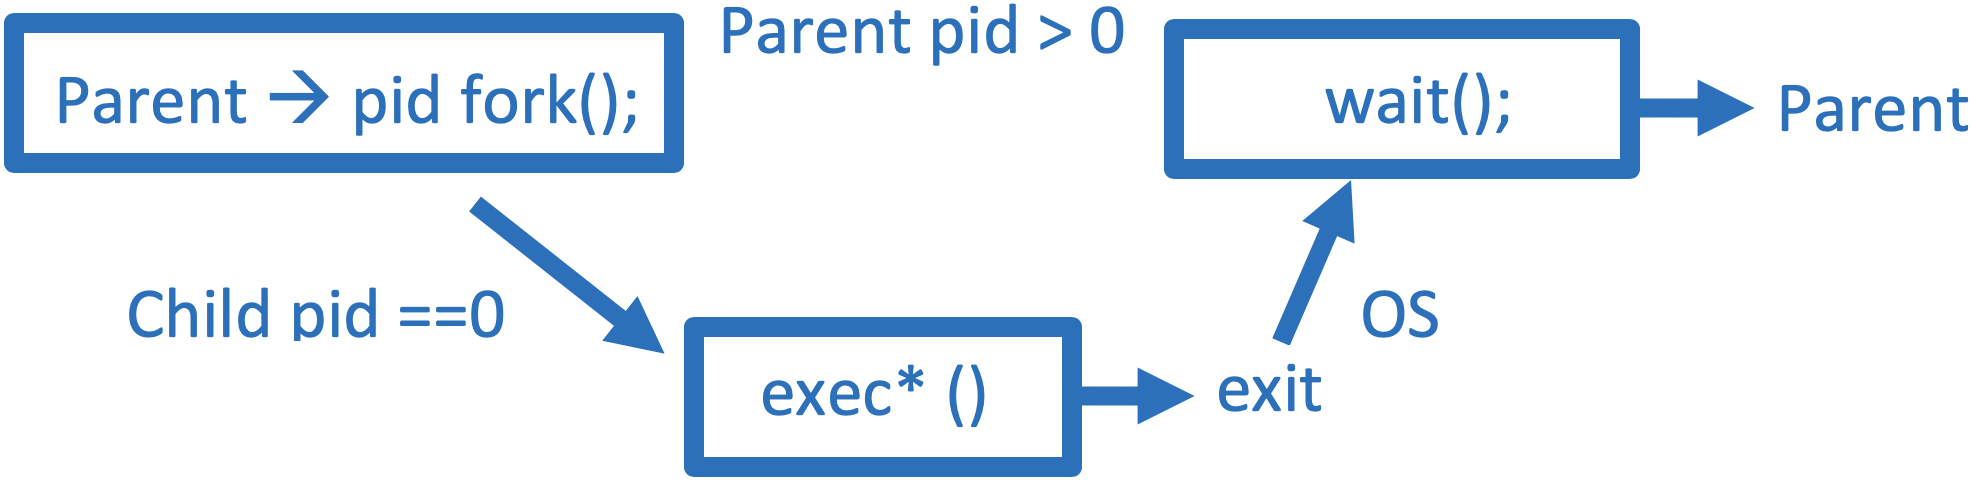
\includegraphics[scale=0.15]{exec.png}
			\end{center}

		\vspace{-7pt}


	\subsubsection{Zombie-Prozess}
	Childprozesse können vom OS erst entfernt werden wenn Parent wait() aufruft $\rightarrow$ Child ist bis dann ein Zombie
			


	\subsubsection{Orphan-Prozess}
	Wird Parentprozess beendet bevor Child fertig ist, hat Child keinen Parent mehr $\rightarrow$ verwaist und kann nicht beendet werden $\rightarrow$ Beim Beenden eines Prozesses werden darum alle Childprozesse an den kill-Prozess [pid = 1] übertragen, dieser ruft kosntant wait() auf um Childprozesse zu töten
		



	\subsubsection{Dauerhafter Zombie-Prozess}
			Bleibt ein Prozess C längere Zeit ein Zombie, bedeutet das, dass sein Parent P wait längere Zeit nicht aufruft. Vermutlich hat P einen Fehler, denn er hat C vergessen $\rightarrow$ C wird an pid 1 übergeben.
	

	\vspace{-5pt}		

	\begin{lstlisting}
unsigned int sleep(unsigned int seconds)
	\end{lstlisting}
	\vspace{-5pt}
	\begin{compactitem}[$\bullet$]
		\item Unterbricht die Ausführung bis die Anzahl der Sekunden ungefähr verstrichen ist. 
		\item Kann aber auch vom System unterbrochen werden.	
	\end{compactitem}
	
	
	
	
	


	
\columnbreak


\section{ELF}

Enthält Informationen für Linker und Loader. 
Enthält ELF Header, Program Header Table (beschreibt Segmente die zur Laufzeit genutzt werden),
Section Header Table (beschreibt Sektionen für den Linker, meist nicht vorhanden bei Objekt-Dateien) und Daten.
Segmente und Sektionen überlappen sich.

Konzepte von OS und Compiler-Toolchain sind aufeinander abgestimmt
Compiler-Toolchain (Linker) erzeugt Executable
OS (Loader) lädt Executable 

ELF kann vielseitig eingesetzt werden
Für zahlreiche Hardware-Architekturen und Betriebssysteme
Für verschiedene Zwischenschritte (Objekte, Bibliotheken, Executables) 

Zwei Views
Execution View mit Segmenten zum Laden in den Hauptspeicher
Linking View mit Sektionen zum Verknüpfen verschiedener Objekt-Dateien

\vspace{-6pt}
\section{Bibliotheken}

Statische Bibliotheken sind Archive von Objekt-Dateien
Linker behandelt statische Bibliotheken wie mehrere Objekt-Dateien




Dynamische Bibliotheken werden erst zur Ladezeit oder Laufzeit des Programms gelinkt
Programm kann Lebenszyklus (teilweise) von Bibliotheken entkoppeln
\vspace{-6pt}
\begin{lstlisting}
void * dlopen (char * filename, int mode)
\end{lstlisting}
\vspace{-6pt}
	\begin{compactitem}[$\bullet$]
		\item Öffnet eine dynamische Bibliothek und gibt ein Handle darauf zurück
		\item mode gibt Art an, wie mit der Bibliothek umgegangen wird
	\end{compactitem}


	\vspace{-6pt}
	\begin{lstlisting}
void * dlsym (void * handle, char * name)
	\end{lstlisting}
	\vspace{-6pt}
		\begin{compactitem}[$\bullet$]
			\item Gibt die Adresse des Symbols "name" aus der mit "handle" bezeichneten Bibliothek zurück
			\item Es werden keine Typinformationen übertragen, man erhält nur eine Adresse 
			\item Es ist also weder klar, ob es sich um Funktionen oder Variablen handelt, noch welche Signatur bzw. welchen Typ diese haben
			\item kann 0 zurückgeben, wenn nicht gefunden
		\end{compactitem}



		\vspace{-6pt}
	\begin{lstlisting}
int dlclose (void * handle)
	\end{lstlisting}
	\vspace{-6pt}
	\begin{compactitem}[$\bullet$]
		\item Schliesst das durch handle bezeichnete, zuvon von dlopen geöffnete Objekt
	\end{compactitem}
		



\textcolor{h}{Linker-Name}: lib + Bibliotheksname + .so (z.B. libmylib.so)\\
\textcolor{h}{SO-Name:} Linker-Name + . + Versionsnummer (z.B. libmylib.so.2)\\
\textcolor{h}{Real-Name:} SO-name + . + Unterversionsnummer (z.B. libmylib.so.2.1) 
	
\vspace{180pt}
.
\vfill
\columnbreak









\section{Threads}
	\begin{compactitem}[$\bullet$]
		\item Threads sind parallel ablaufende Aktivitäten innerhalb eines Prozesses
		\item Threads haben auf alle Ressourcen im Prozess gleichermassen Zugriff
		\item In Linux jeder Thread Kopie des PCB seines Prozesses, aber mit eigenem Kontext
	\end{compactitem}
	
	
	\subsubsection{Amdahls Regel}
	$n$ n-Prozessoren\\
	T Ausführungszeit, wenn komplett seriell ausgeführt\\
	T' Zeit, wenn max. parallelisiert\\
	T$_{s}$ Zeit, serieller Anteil\\
	T - T$_{s}$ Zeit, parallelisierbarer Anteil\\
	$\frac{T - T_{s}}{n}$  Parallel-Anteil verteilt auf n-Prozessoren\\
	s $=$ $\frac{T}{T_{s}}$ serieller Anteil Algorithmus
	
	\subsubsection{Speedup-Faktor}
	$f \leq \frac{T}{T'} = \frac{T}{T_{s} + \frac{T - T_s}{n}} = \frac{T}{s * T + \frac{T - s * T}{n}} = \frac{T}{s * T + \frac{1 - s}{n} * T} = \frac{1}{s + \frac{1 - s}{n}}$

	Ist maximal $f$-mal schneller, wenn parallel




	\begin{lstlisting}
int pthread_create (pthread_t * thread_id, 
pthread_attr_t const * attributes, void * 
(* start_function ) ( void *), void * argument)
	\end{lstlisting}
	\vspace{-6pt}
	\begin{compactitem}[$\bullet$]
		\item Erzeugt Thread, bei Erfolg 0 zurück
		\item neue ID im Out-Parameter thread\_id
	\end{compactitem}
	
	\vspace{-2pt}
	\drule{\linewidth}{1pt}

	Ein Thread \textcolor{h}{lebt solange bis} folgenden Bedingung:
		\begin{compactitem}[$\bullet$]
			\item Er springt aus der Funktion start\_function zurück
			\item Er ruft pthread\_exit auf
			\item Ein anderer Thread ruf pthread\_cancel auf
			\item Sein Prozess wird beendet
		\end{compactitem}

	\vspace{-5pt}
					
				
	\begin{lstlisting}
void pthread_exit (void *return_value)
	\end{lstlisting}
	\vspace{-5pt}
	Beendet den Thread und gibt den return\_value zurück.

	\vspace{-5pt}

	\begin{lstlisting}
int pthread_cancel (pthread_t thread_id)
	\end{lstlisting}
	\vspace{-5pt}
	Sendet Anforderung, dass der Thread mit thread\_id beendet werden soll. Wartet nicht, dass der Thread tatsächlich beendet wurde.

	\vspace{-5pt}

	\begin{lstlisting}
int pthread_detach (pthread_t thread_id)
	\end{lstlisting}
	\vspace{-5pt}
	Entfernt den Speicher, den ein Thread belegt hat, falls dieser bereits beendet wurde. Beendet den Thread aber nicht!

	\vspace{-5pt}

	\begin{lstlisting}
int pthread_join (pthread_t thread_id, void ** return_value )
	\end{lstlisting}
	\vspace{-5pt}
	Wartet solange, bis der Thread mit thread\_id beendet wurde. Ruft pthread\_detach auf.
	
	\vspace{-5pt}

	\begin{lstlisting}
pthread_t pthread_self (void)
	\end{lstlisting}
	\vspace{-5pt}
	Gibt die ID des gerade laufenden Threads zurück.

	\vspace{-5pt}

	\begin{lstlisting}
int pthread_key_create (pthread_key_t *key , void (* destructor )( void *))	
	\end{lstlisting}
	\vspace{-5pt}
		\begin{compactitem}[$\bullet$]
			\item Erzeugt neuen Key im Out-Parameter key. 
			\item pthread\_key\_t ist eine opake Datenstruktur. 
			\item Jeden Thread/Key hält OS Wert vom Typ void * 
			\item Dieser Wert immer mit NULL initialisiert. 
			\item OS ruft destructor am Ende des Threads mit thread Wert auf, wenn nicht NULL 
		\end{compactitem}
	
	
		\vspace{-5pt}
	
		
	\begin{lstlisting}
int pthread_key_delete (pthread_key_t key)
	\end{lstlisting}
	\vspace{-5pt} 
	\begin{compactitem} [$\bullet$]
		\item Entfernt den Key und die entsprechenden Values aus allen Threads. 
		\item Der Key darf nach diesem Aufruf nicht mehr verwendet werden. 
		\item Das Programm muss dafür sorgen, sämtlichen Speicher freizugeben, der eventuell zusätzlich alloziert worden war. 
		\item Gib 0 zurück, wenn alles OK war, sonst einen Fehlercode.
	\end{compactitem}

	\vspace{-5pt}


	\begin{lstlisting}
int pthread_setspecific (pthread_key_t key,
const void * value ) void * pthread_getspecific 
(pthread_key_t key)
	\end{lstlisting}
	\vspace{-5pt}
		\begin{compactitem}[$\bullet$]
			\item Schreibt bzw. liest den Wert, der mit dem Key in diesem Thread assoziiert ist. 
			\item Typischerweise verwendet man den Wert als Pointer auf einen Speicherbereich
		\end{compactitem}
				


\section{Scheduling}
	Zustände, Thread befindnen kann:\\
	\textcolor{h}{running:} aka Prozessor-Burst, Thread ist aktiv\\
	\textcolor{h}{ready:} alle Threads die aktiv sein könnten\\
	\textcolor{h}{waiting:}wartet auf Externes Ereignis (Input)\\
	OS macht übergänge.
	
	\vspace{-2pt}
	\drule{\linewidth}{1pt}

	\textcolor{h}{Ready-Queue} Datenstruktur (bspw Tree) in der ready Threads warten\\
	\textcolor{h}{Standby} Prozessor schaltet in einen Energiespaarmodus wenn alle Threads warten\\
	\textcolor{h}{Kooperativ} Jeder Thread entscheidet	selbst, wann er den Prozessor abgibt\\
	\textcolor{h}{Präemptiv} Scheduler entscheidet, wann einem Thread der Prozessor entzogen wird\\
	\textcolor{h}{Parallel} n Threads benötigen n Prozessoren\\
	\textcolor{h}{Quasiparallel} n Threads auf $<$n Procs aufgeteilt\\
	\textcolor{h}{Prozessor-Burst} Intervall, in dem ein Thread den Prozessor in einem parallelen System voll belegt\\
	\textcolor{h}{I/O-Burst} Intervall, in dem ein Thread den Prozessor nicht benötig\\

	\vspace{-4pt}
	\subsubsection{Anforderungen an Scheduler}
	\textcolor{h}{Closed-System} perfekt optimiert (Embedded)\\
	\textcolor{h}{Open-System} OS, wird an Verwender angepasst

	\vspace{-2pt}
	\drule{\linewidth}{1pt}
	\textcolor{h}{Durchlaufzeit} Zeit vom Starten bis Ende Thread\\
	\textcolor{h}{Antwortzeit} Zeit vom Empfang eines Requests bis die Antwort zur Verfügung steht\\
	\textcolor{h}{Wartezeit} Zeit, Thread in Ready-Queue\\
	\textcolor{h}{Durchsatz} Anz. Threads pro Intervall bearbeitet\\
	\textcolor{h}{Prozessor-Verwendung:} Prozentsatz des Prozessors (Verwendung zu idle)\\

	\vspace{-23pt}
	\begin{center}
		
\includegraphics[scale =.155]{Infobar.png}
		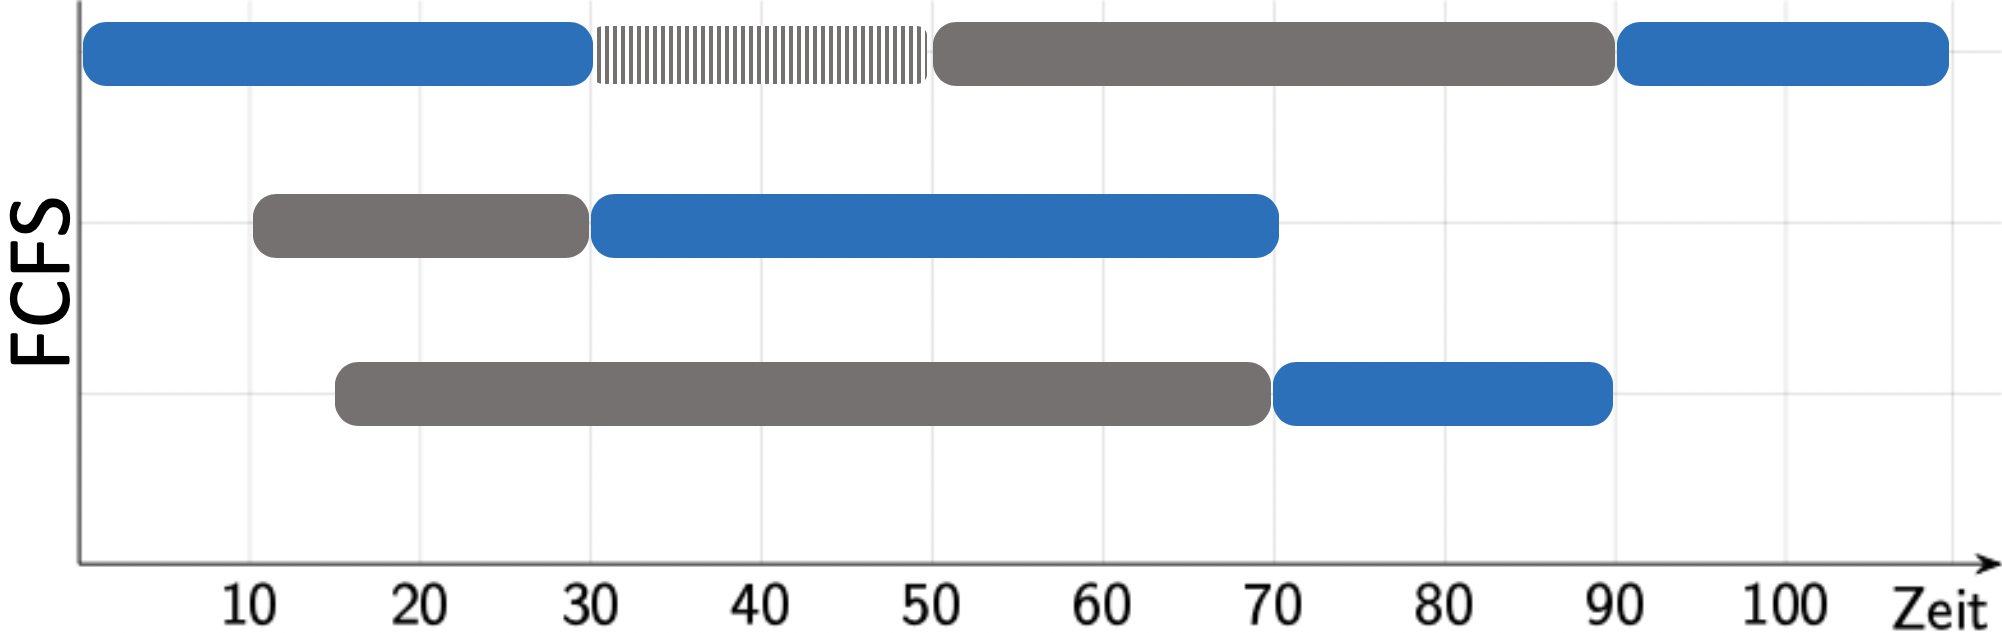
\includegraphics[scale =.155]{FCFS.png}
		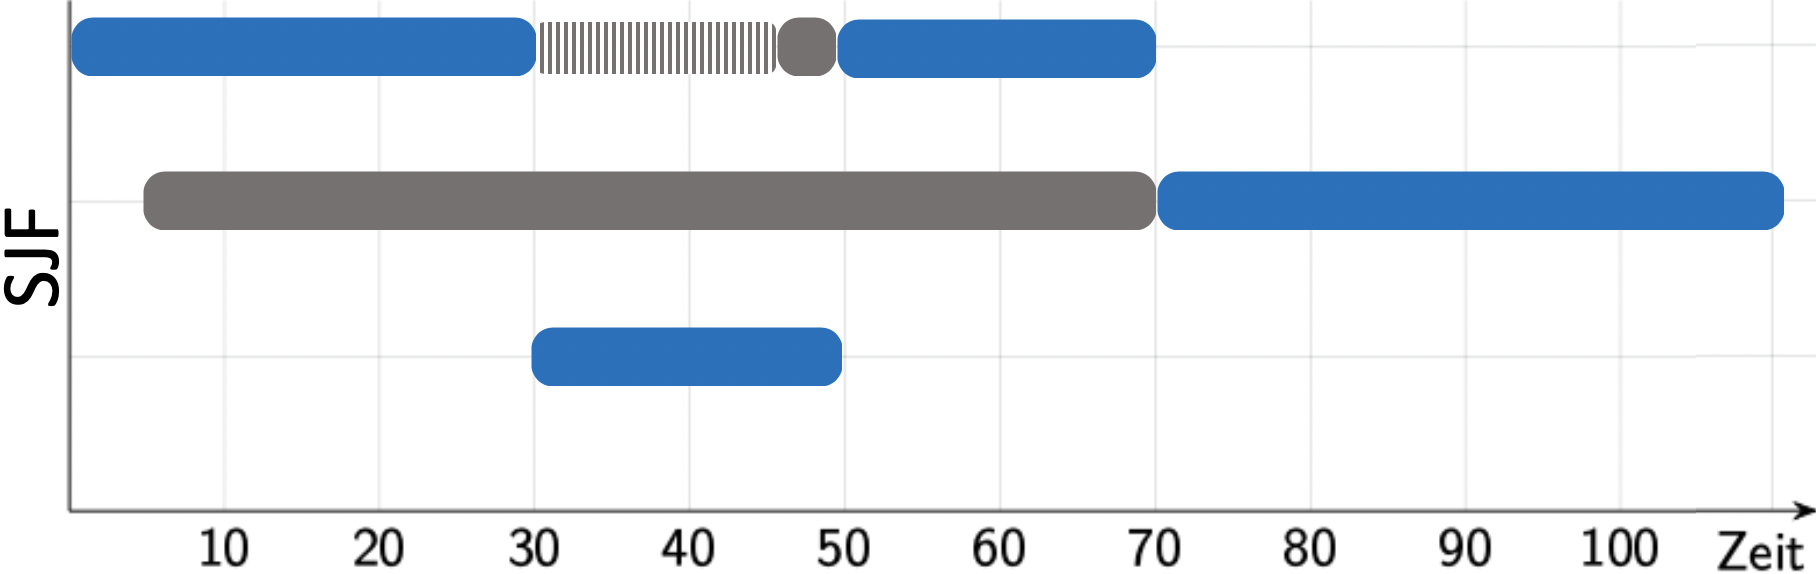
\includegraphics[scale =.155]{SJF.png}
		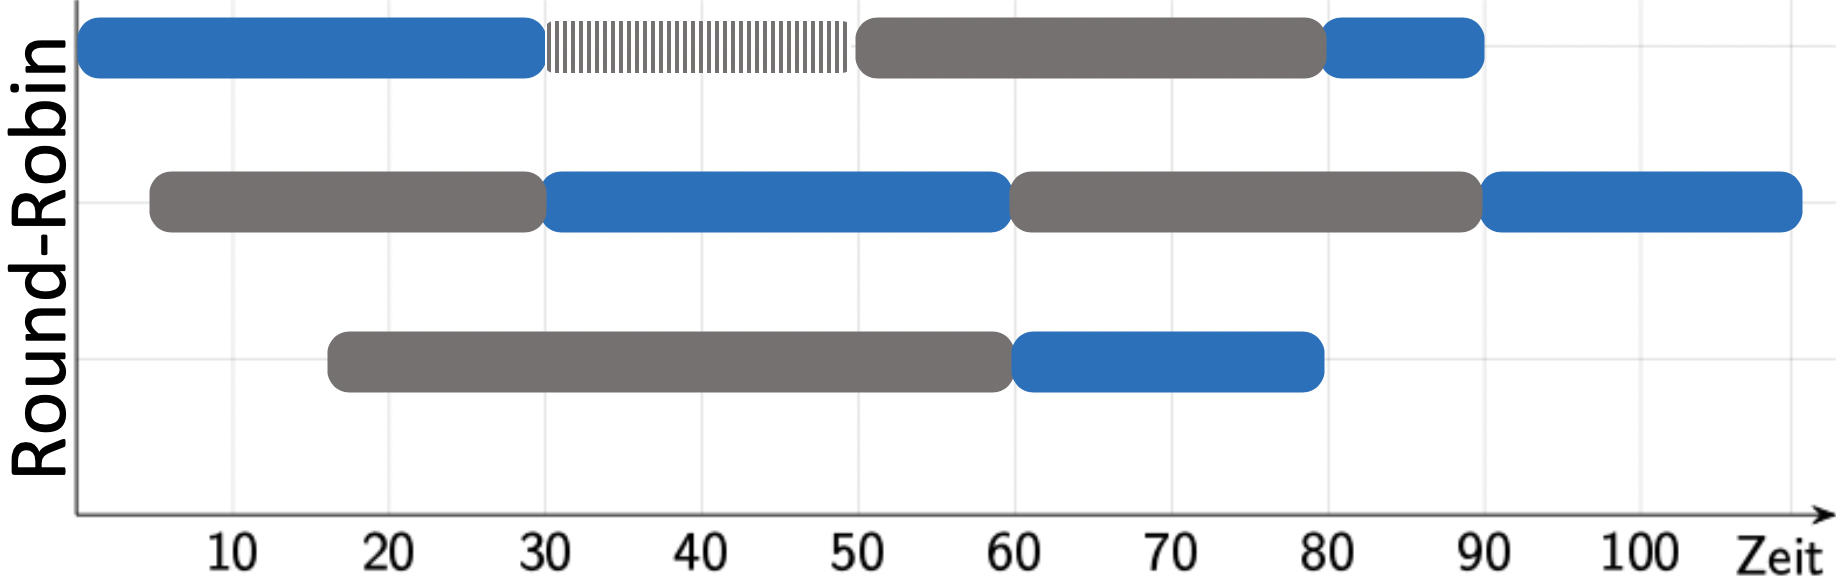
\includegraphics[scale =.155]{RoundRobin.png}
	\end{center}

	\vspace{-10pt}
	Jeder Prozess / Thread hat Nice-Wert (-20 bis + 19) Umso kleiner der Wert, umso bevorzugter.

	

	
\vspace{-5pt}



\section{Mutexe und Semaphore}

\textcolor{h}{Abschalten von Interrupts} unpraktisch \& gefährlich, OS kann Thread nicht mehr unterbrechen


\subsubsection{Semaphore}

\begin{compactitem}[$\bullet$]
	\item Ein Semaphor enthält einen Zähler z $\geq$ 0
	\item Auf dem Semaphor wird nur über spezielle Funkionen zugegriffen\\
	\textcolor{h}{Post} Erhöht z um 1\\
	\textcolor{h}{Wait} Wenn z $>$ 0: Verringert z um 1 und setzt Ausführung fort\\
	\textcolor{h}{Wait} Wenn z $=$ 1 : Versetzt den Thread in waiting, bis ein anderer Thread z erhöht
\end{compactitem}
Der \textcolor{h}{Producer wartet} darauf, dass mindestens ein Element frei oder gefüllt ist. 
Consumer und Producer geben sich gegenseitig Semaphore frei.


\subsubsection{Priority Inversion}
Thread mit Prio zwischen haltendem/wartendem arbeitet.

\subsubsection{Priority Inheritance}
Thread, der Ressource hält, erhält die höchste Priorität aller Threads, die auf diese Ressource warten.


\subsubsection{Mutexe}
\begin{compactitem}[$\bullet$]
	\item Ein Mutex hat einen binären Zustand z, der nur durch zwei Funktionen verändert werden kann:
	\item \textcolor{h}{Acquire} Wenn z = 0: Setzt z auf 1 und fahre fort
	\item \textcolor{h}{Acquire} Wenn z = 1 : Blockiere den Thread solange, bis z = 0
	\item \textcolor{h}{Release} Setzt z = 0
	\item Kann durch einen Semaphor mit Beschränkung von z auf 1 realisiert werden 
	\item Acquire und Release heissen auch Lock und Unlock
\end{compactitem}

\vspace{-5pt}






\section{Signale und Sockets}
	Signale ermöglichen es, einen Prozess von aussen zu unterbrechen\\
	verhält sich das OS, als ob ein Interrupt geschickt wurde


	\subsubsection{Programmfehler}
	\begin{compactitem}[$\bullet$]
		\item \textcolor{h}{SIGFPE} Fehler in arithmetischer Operation
		\item \textcolor{h}{SIGILL} Ungültige Instruktion 
		\item \textcolor{h}{SIGSEGV} Ungültiger Speicherzugriff
		\item \textcolor{h}{SIGSYS} Ungültiger Systemaufruf
	\end{compactitem}

	\subsubsection{Prozesse Abbrechen}
	\begin{compactitem}[$\bullet$]
		\item \textcolor{h}{SIGTERM} höfliche Anfrage
		\item \textcolor{h}{SIGINT} Ctrl-C drücken
		\item \textcolor{h}{SIGQUIT} Wie SIGINT aber anormal, Ctrl-\ 
		\item \textcolor{h}{SIGABRT} Wie SIGQUIT (vom Prozess an sich selbst geschickt)
		\item \textcolor{h}{SIGKILL} kann der Prozess nicht blockieren
	\end{compactitem}


	\subsubsection{Stop und Continue}
	\begin{compactitem}[$\bullet$]
		\item \textcolor{h}{SIGTSTP} Zustand stopped, ähnlich waiting
		\item \textcolor{h}{SIGSTOP} Wie SIGTSTP, kann nicht ignoriert
		\item \textcolor{h}{SIGCONT} Setzt den Prozess fort
	\end{compactitem}

	\vspace{-3pt}
	\begin{lstlisting}
int sigaction(int sig, struct sigaction *new,
	struct sigaction *old)		
	\end{lstlisting}

	\vspace{-5pt}

\subsubsection{Pipes}
	Pipes ermöglichen Kommunikation über Prozess-Grenzen hinweg

	\vspace{-5pt}

	\begin{lstlisting}
int pipe(int fd [2])		
	\end{lstlisting}

	\vspace{-5pt}

	Erzeugt eine Pipe und zwei File-Deskriptoren, die in fd abgelegt werden\\
	Pipe lebt solange, wie sie in einem Prozess geöffnet bleibt

	\vspace{-3pt}
	\drule{\linewidth}{1pt}

\textcolor{h}{lesen aus pipe:}
Aus einer Pipe kann mit read gelesen werden, als ob sie eine Datei wäre Sind keine Daten in der Pipe, blockiert read, bis Daten hineingeschrieben werden.\\
Lesender Prozess sollte write end schliessen, schreibender Prozess read end!



\subsubsection{Sockets}
eine Abstraktion über Kommunikationsmechanismen 

Ein \textcolor{h}{Client verwendet einen Socket}:
\begin{compactenum}[1.]
	\item Verbindung unter Angabe einer Adresse aufbauen: connect
	\item Senden von Daten (z.B. eine Anfrage): send oder write
	\item Empfangen von Daten (z.B. eine Antwort): recv oder read
	\item Schliessen der Verbindung: close
\end{compactenum}

	$\rightarrow$ Senden und Empfangen sind jeweils optional und können beliebig oft wiederholt werden.

Ein \textcolor{h}{Server verwendet einen Socket}:
\begin{compactenum}[1.]
	\item Festlegen einer nach aussen sichtbaren Adresse: bind
	\item Bereitstellen einer Queue zum Sammeln von Verbindungsanfragen von Clients: listen 
	\item Erzeugen eine Verbindung auf Anfrage von Client: accept (erzeugt neuen Socket) 
	\item Empfangen von Daten (z.B. eine Anfrage): recv oder read 
	\item Senden von Daten (z.B. eine Antwort): send oder write 
	\item Schliessen der Verbindung: close
\end{compactenum}
	$\rightarrow$	Senden und Empfangen sind jeweils optional und können beliebig oft wiederholt werden.



\section{Message Passing}

\textcolor{h}{Send} kopiert Nachricht aus dem Prozess\\
\textcolor{h}{Recive} kopiert Nachricht in den Prozess\\
\textcolor{h}{Direkt} Sender muss Empfänger kennen\\
\textcolor{h}{Symmetrisch} Empf. muss Sender kennen\\
\textcolor{h}{Assymetrisch} Empfänger erhält eine msg-id beim Abfragen neuer Nachrichten\\
\textcolor{h}{Indirekt} funktioniert via Datenstruktur die beide kennen (Message-Queue)\\
\textcolor{h}{synchron} Message-Passing blockierend\\
\textcolor{h}{asynchron} nicht-blockierend \\
\textcolor{h}{Rendevouz} Sender \& Empfänger blockieren

\vspace{-7pt}

\section{Shared Memory}
\textcolor{h}{Selbes Frame} wird für mehrere Prozesse benutzt\\
\textcolor{h}{Synchronisierung} nötig (e.g. via Mutex)\\
\textcolor{h}{Pointer} müssen relativ zu einer Anfangsaddr sein



\vspace{-7pt}

\section{Unicode}

\textcolor{h}{ASCII:}\\
128 Zeichen $\rightarrow$ 7 Bit, 00 bis 7F\\
Viele unabhängige Erweiterungen mit 8 Bit (ISO-XYZ)

\textcolor{h}{UTF:}
\begin{compactitem}[$\bullet$]
	\item D800 - DFFF keine gültigen Code-Points (wegen UTF-16)
	\item Code-Point (CP): Nummer eines Zeichen (max 21 Bit)
	\item Code-Unit (CU): Einheit, um Zeichen darzustellen
	\item UTF-32: CU 32 Bit, CP 1 CU
	\item UTF-16: CU 16 Bit, CP 1-2 CU
	\item UTF-8: CU 8 Bit, CP 1-4 CU
	\item UTF-16 und UTF-32 müssen Endianness beachten
\end{compactitem}



\subsubsection{Bsp.}
\vspace{-2pt}
\begin{tabular}{c p{.82cm} | r | r}
	\hline
	&CP&UTF-32BE&UTF-32LE\\
	\hline
	A&41&00 00 00 41&41 00 00 00\\
	ä&E4&00 00 00 E4&E4 00 00 00\\
	$\alpha$&3B1& 00 00 03 B1& B1 03 00 00\\
	$\breve{a}$&1EB7&00 00 1E B7& B7 1E 00 00\\
	$\wp$&10330& 00 01 03 30& 30 03 01 00 \\
	\hline
	
\end{tabular}


\begin{tabular}{ r | r | r}
	\hline
	UTF-8&UTF-16BE&UTF-16LE\\
	\hline
	41&00 41&41 00 \\
	C3 A4&00 E4&E4 00\\
	CE B1&03 B1&B1 03\\
	E1 BA B7&1E B7&B7 1E\\
	F0 90 8C B0& D8 00 DF 30&00 D8 30 DF\\
\hline
	
\end{tabular}


\subsubsection{Berechnung UTF-8:}
CP in \textcolor{h}{[80, 7FF]:} Bis zu 11 sign. Bits\\
(p0-5 + 80; 6-10 + C0)\\
CP in \textcolor{h}{[800, FFFF]:} Bis zu 16 sign.\\
(p0-5 + 80; 6-11 + 80; 12-15 + E0)\\
CP in \textcolor{h}{[1'0000, 10'FFFF]:} Bis zu 21 sig.\\
(p0-5 + 80; 6-11 + 80; 12-17 + 80; 18-20 + F0)\\

\begin{compactenum}[1.]
	\item CP Binär schreiben
	\item Length ermitteln
	\item 0-en vorne auffüllen
	\item neue p's errechnen (p0-5=) in hex
	\item neue u's errechnen (p's + hex addon)
\end{compactenum}

\subsubsection{Berechnung UTF-16:}
\begin{compactenum}[1.]
	\item wenn CP [0, FFFF] $\rightarrow$ direkt schreiben
	\item wenn CP [1'0000, 10'FFFF]:
	\item Q = CP - $10000_{hex}$
	\item Q binär schreiben, 0en auffüllen
	\item U1 = $(q0-q9)_{hex}$ + D800
	\item U0 = $(q10-q19)_{hex}$ + DC00
	\item BE = U1 U0 (D8 00 DF 30)
	\item LE = U0 U1 (00 D8 30 DF)
\end{compactenum}







\vfill
\columnbreak



\section{Dateisystem ext2}

\textcolor{h}{Partition:} Teilbereich des Datenträgers\\
\textcolor{h}{Volume:} Datenträger oder Partition\\
\textcolor{h}{Sektor:} Kleinste logische Untereinheit eines Volumes (traditionell 512 Bytes, heute 4 KB mit Header, Daten und Error-Correction-Codes)\\
\textcolor{h}{Format:} Layout der logischen Strukturen auf dem Datenträger\\
\textcolor{h}{Block:} Mehrere aufeinanderfolgende Sektoren, gesamte Volume ist in Blöcke aufgeteilt\\
\textcolor{h}{Speicher:} nur in Form von Blöcken alloziert

\textcolor{h}{Inodes}: 
\begin{compactitem}[$\bullet$]
	\item enthält alle Metadaten über Datei (ausser Name + Pfad)
	\item Fixe Grösse je Volume: Zweierpotenz, mind. 128 Byte, max. 1 Block
	\item verweist auf die Blöcke, die Daten für die Datei enthalten
	\item Enthält ein Array i\_block mit 15 Einträgen zu je 32 Bit
\end{compactitem}

\textcolor{h}{Indirekter Block}: \\
Enthält 32-Bit Nummern der Blöcke der Datei ab Block 12\\
Blockgrösse 1024 Byte $\rightarrow$ 256 Blocknummern

\textcolor{h}{Doppelt indirekter Block}:
Enthält Nummern von indirekten Blöcken 
Blockgrösse 1024 $\rightarrow$ 256 * 256 Blöcke $\rightarrow$ 65536 Blöcke referenziert

\textcolor{h}{Dreifach indirekter Block}:
Enthält Nummern von doppelt indirekten Blöcken 
Blockgrösse 1024 $\rightarrow$ 256 * 256 * 256 = 16M Blöcke referenziert


\textcolor{h}{File-Holes:}\\
Bereiche in der Datei, in der nur Nullen stehen


\textcolor{h}{Verzeichnisse:} (Entry 8-263 Bytes vielfaches 4By)
\begin{compactitem}[$\bullet$]
	\item 4 Bytes Inode $\bullet$2 Byte Length of Entry
	\item 1 Byte Length of Name $\bullet$0-255 Byte Name
	\item 1 Byte File Type (1=Datei, 2=Verzeichnis, 7=Symbolischer Link), 
\end{compactitem}

\textcolor{h}{Links:}

\textbf{Hardlink:} gleicher Inode, verschiedene Pfade
\textbf{Symbolischer Link:} Datei enthält Pfad anderer Datei

\textcolor{h}{Blockgruppe:}
\begin{compactitem}[$\bullet$]
	\item Mehrere aufeinanderfolgende Blöcke
	\item Bei Blockgrösse 4 KB sind bis zu 32 K Blöcke in einer Gruppe
	\item Block 0: Kopie des Superblocks 
	\item Block 1 bis n: Kopie der Gruppendeskriptorentabelle 
	\item Block n + 1: Block-Usage-Bitmap mit einem Bit je Block der Gruppe 
	\item Block n + 2: Inode-Usage-Bitmap mit einem Bit je Inode der Gruppe 
	\item Block n + 3 bis n + m + 2: Tabelle aller Inodes in dieser Gruppe 
	\item Block n + m + 3 bis Ende der Gruppe: Blöcke der eigentlichen Daten
\end{compactitem}

\textcolor{h}{Superblock}
Enthält alle Metadaten über das Volume, Startet immer an Byte 1024\\
1 x pro Blockgruppe!

\textcolor{h}{Gruppendeskriptor:}
32 Byte Beschreibung einer Blockgruppe


\textcolor{h}{Gruppendeskriptortabelle}
Ein Gruppendeskriptor je Gruppe\\
Benötigt selbst 32 * n Anzahl Bytes\\
Anzahl Sektoren = 32 * n / Sektorgrösse\\
Folgt direkt auf Superblock


\textbf{Berechnungen:}
\begin{compactenum}[1.]
	\item Dateigrösse $\rightarrow$ $2^{x}$
	\item $2^{x}$ - Blockgrösse = Anz. Blöcke/Einträge
	\item Einträge in hex umwandeln
	\item "0 $\rightarrow$ Startadresse,..." (bis B)
	\item "C $\rightarrow$ <Adresse> indirekter Block"
	\item "<Adresse> indirekter Block.0 $\rightarrow$ Adresse C"
\end{compactenum}







\vspace{-5pt}


\section{Dateisystem ext4}
\begin{compactitem}[$\bullet$]
\item Inodes mit 256 Bytes statt 128, 
\item Gruppendeskriptor 64 statt 32, 
\item Blockgrösse bis 64KB
\item Inodes verwalten Blöcke mit Extent Trees (12Byte, max. 5 Ebenen)
\end{compactitem}


\textcolor{h}{Extent:} (12 Byte)
\begin{compactitem}[$\bullet$]
	\item logischen \& physischen Blocknummer (4/6 B)
	\item Anzahl Blöcke (2 B, signed)
	\item Datei muss mehr als einen Extent umfassen können
\end{compactitem}



Im \textcolor{h}{Inode:}\\
1. Element Extent Tree Header, dann 4 x Extends (entweder innere (Level > 0) oder äussere Knoten (Level = 0))

Für \underline{mehr als 4 Extents} braucht man einen \underline{zusätzlichen Block}. 
Deshalb sind die ersten 12 Byte kein Extent, sondern der Extent Tree Header

Ein innerer Knoten beschreibt einen Block, der selbst wieder Baumelemente enthält: Header und Knoten oder Extents.



\textcolor{h}{Index Nodes}
Index-Node spezifiziert einen Block, der Extents enthält
Physische Blocknummer des Blocks, auf den der Index-Node verweist

\textbf{Berechnungen:}
\begin{compactenum}[1.]
	\item "0 $\rightarrow$ (Anz. Einträge, Tiefe) (Header)"
	\item wenn mehr als 4 E $\rightarrow$ Index Node + Header2
	\item sonst: "1 $\rightarrow$ (log., phy., Anz. Blöcke) (Extent)"
\end{compactenum}

\textcolor{h}{\textbf{Jounaling}}

\textbf{Idee} Speicherbereich auf Festplatte reservieren, auf den Daten schnell zwischengespeichert werden können. Schreibt nur die Transaktion, die zu erfolgen. Inkonsistenzen schneller überprüfen, da nicht alle Metadaten verifiziert werden müssen.\\
\textbf{mode Journal} Daten werden komplett, ins Journal geschrieben, dann richtig, dann aus dem Journal entfernt.\\
\textbf{mode Ordered} Nur Metadaten im Journal. Transaktion $\rightarrow$ Dateiinhalte $\rightarrow$ Commit. Dateien haben sicher richtigen Inhalt nach Commit, aber nicht optimale Performance.\\
\textbf{mode Writeback} Nur Metadaten im Journal. Commit und Dateiinhalte schreiben in beliebiger Reihenfolge.
 
 
\vspace{-5pt}
 

\section{X Window System}

\textcolor{h}{X Window System:}
\begin{compactitem}[$\bullet$]
\item Fensterhierarchie, verteilt Nachrichten
\end{compactitem}

\textcolor{h}{Window Manager:}
\begin{compactitem}[$\bullet$]
\item Applikationsfenster mit Titelleiste, Umrandung, Knöpfen	
\item Fenster verschieben, in der Grösse ändern, etc.
\item sendet ein ClientMessage Event an App
\end{compactitem}


\textcolor{h}{Display:} Screen/Maus/Tastatur\\
\textcolor{h}{X Client:} Applikation, die Display nutzen will\\
\textcolor{h}{X Server:} Softwareteil des X Window System, der ein Display ansteuert

\textbf{Requests:} Dienstanforderungen\\
Client $\rightarrow$ Server ($\rightarrow$"liefere aktuelle Fensterposition" (Request Buffer))

\textbf{Replies:} Antworten auf Requests\\
Client $\leftarrow$ Server

\textbf{Events:} spontane Ereignismeldungen\\
Client $\leftarrow$ Server ($\rightarrow$ Benutzereingaben via Tastatur (doppelt gepuffert))

\textbf{Errors:} Fehlermeldungen auf vorangegangene Requests, Client $\leftarrow$ Server

\textcolor{h}{Client} muss vorher festlegen, welche Ereignistypen empfangen will (XSelectInput())\\
\textcolor{h}{X Ressource:} Server-seitige Datenhaltung zur Reduktion des Netzwerkverkehrs (im Auftrag von Clients)

\textcolor{h}{Atom} ist die ID eines Strings, der für Meta-Zwecke benötigt wird\\
Anstelle von "WM\_DELETE\_MESSAGE" verwendet man intern Atom 5

\textcolor{h}{WM\_PROTOCOLS}\\
X Standard definiert eine Anzahl an Protokollen, die der Window Manager verstehen soll.\\
Client kann sich für Protokolle registrieren.\\
Dazu muss er im Property WM\_PROTOCOLS die Liste der Atome der Protokollnamen speichern

\textcolor{h}{WM\_DELETE\_WINDOW}
Window-Close-Event, Server $\rightarrow$ Client




\end{multicols*}





% \appendix

% List of figures
\listoffigures

% List of tables
\listoftables



\end{document}